\chapter{Global Minimum Cut}

A cut is a way of breaking a graph into two pieces. So far, when we have talked about cuts at all, we have had two distinguished vertices in mind: a source $s$ and a sink $t$, and we wanted the cheapest set of edges whose removal disconnects $t$ from $s$. That is the \emph{$s$--$t$ min-cut}, and it is the dual of maximum flow (Chapter~12). This chapter asks a different question, one with no fixed endpoints at all:

\begin{quote}
What is the cheapest set of edges whose removal disconnects the graph into two nonempty pieces?
\end{quote}

This is the \emph{global} minimum cut. It is the weakest point of a network: the smallest amount of capacity you would have to sever to split it in two, no matter where the split happens to fall. The freedom to choose both sides of the cut makes the problem feel harder than $s$--$t$ flow, yet some of the most elegant algorithms in all of combinatorial optimization live here. We will see two of them: a deterministic algorithm of Stoer and Wagner that finds the answer with a sequence of greedy ``most-tightly-attached'' orderings, and a randomized algorithm of Karger that repeatedly contracts a random edge and, astonishingly, lands on the min-cut with non-trivial probability. The Karger--Stein refinement turns that into one of the fastest known min-cut algorithms, and its analysis is a beautiful piece of elementary probability.

\chapterline

\section{The problem, precisely}

Let $\Gph=(V,E)$ be a connected undirected graph with $n=\abs{V}$ vertices and $m=\abs{E}$ edges, and let each edge $e$ carry a nonnegative weight $w(e)\ge 0$ (for unweighted graphs read $w(e)=1$). A \emph{cut} is a partition of the vertices into two nonempty sets $(S,\bar S)$ with $\bar S = V\setminus S$ and $\emptyset \neq S \neq V$. The \emph{weight} (or capacity) of the cut is the total weight of the edges crossing it:
\[
  w(S,\bar S) \;=\; \sum_{\substack{e=\{u,v\}\in E\\ u\in S,\ v\in\bar S}} w(e).
\]

\begin{definition}[Global minimum cut]\label{ch11:def-mincut}
The \emph{global minimum cut} of $\Gph$ is a cut of minimum weight over all partitions $(S,\bar S)$. Its value is
\[
  \lambda(\Gph) \;=\; \min_{\emptyset\neq S\subsetneq V} w(S,\bar S).
\]
For unweighted graphs $\lambda(\Gph)$ is the \emph{edge connectivity}: the fewest edges whose deletion disconnects $\Gph$.
\end{definition}

\begin{intuitionbox}
Picture the graph as a sheet of fabric and each edge as a thread of a certain thickness $w(e)$. A cut is a pair of scissors slicing the fabric into two nonempty pieces; its cost is the total thickness of the threads you sever. The global min-cut is the place where the fabric is most flimsy. The $s$--$t$ version forces you to keep two named points on opposite sides of the slice; the global version lets the scissors fall anywhere, so $\lambda(\Gph) \le w(S,\bar S)$ for \emph{every} cut, in particular every $s$--$t$ cut.
\end{intuitionbox}

\paragraph{Why not just run max-flow?}
You can reduce global min-cut to $s$--$t$ min-cut. Fix any single vertex $s$ (it must end up on one of the two sides). Then the global min-cut is the cheapest $s$--$t$ cut over all choices of the other terminal $t$:
\[
  \lambda(\Gph) \;=\; \min_{t\neq s}\; \big(\text{$s$--$t$ min-cut}\big).
\]
The fixed $s$ lands on some side; whichever real vertex $t$ sits on the opposite side certifies that $s$--$t$ cut, and the cheapest over $t$ is the global optimum. So $n-1$ max-flow computations suffice. With a good flow algorithm this is roughly $\Oh(n\cdot mn) = \Oh(mn^2)$, and Hao--Orlin sharpens it to a single ``stack of flows'' run in $\Oh(mn\log(n^2/m))$. But two direct combinatorial algorithms beat the naive reduction without ever computing a flow, and they are the subject of this chapter.

\begin{focusbox}
Three facts we will lean on repeatedly:
\begin{enumerate}
  \item $\lambda(\Gph)$ is at most the minimum weighted degree $\delta = \min_v \sum_{e\ni v} w(e)$, because isolating a single minimum-degree vertex is a cut.
  \item Every cut $(S,\bar S)$ separates \emph{some} pair $u\in S$, $v\in \bar S$. So the global cut equals $\min_{u,v}$ of the $u$--$v$ min-cut over all $\binom{n}{2}$ pairs --- but we will never need all pairs.
  \item Contracting an edge $\{u,v\}$ (merging $u$ and $v$ into one vertex, summing parallel edges, dropping the self-loop) can only destroy cuts that separated $u$ from $v$. Cuts that kept $u,v$ together survive unchanged. This single observation powers Karger's algorithm.
\end{enumerate}
\end{focusbox}

\begin{historybox}
The global min-cut problem is old, but its clean combinatorial algorithms are surprisingly recent. Through the 1980s the standard route was $n-1$ max-flow computations; Hao and Orlin (1992) showed how to share work across them. Then in 1992 Nagamochi and Ibaraki, and independently in their 1997 paper Stoer and Wagner, found a flow-free deterministic algorithm of striking simplicity. Meanwhile David Karger, as a Stanford graduate student, proposed random edge contraction in 1993; with Clifford Stein in 1996 he refined it to an $\Oh(n^2\log^3 n)$ algorithm. Karger's 2000 tree-packing algorithm reached near-linear time $\Oh(m\log^3 n)$, and the saga continued into the 2020s with deterministic near-linear algorithms (Henzinger--Rao--Wang, Li). We cover the two foundational gems: Stoer--Wagner and Karger(--Stein).
\end{historybox}

\section{A tiny graph to keep in mind}

We will trace every algorithm on the same small weighted graph, so keep this picture handy. It is the example from Stoer and Wagner's paper.

\begin{figure}[H]
\centering
\begin{tikzpicture}[every node/.style={circle,draw,fill=blue!8,minimum size=7mm,inner sep=1pt,font=\small},
  thick,>=Stealth]
  \node (1) at (0,2)   {1};
  \node (2) at (2,2)   {2};
  \node (3) at (4,2)   {3};
  \node (4) at (6,2)   {4};
  \node (5) at (0,0)   {5};
  \node (6) at (2,0)   {6};
  \node (7) at (4,0)   {7};
  \node (8) at (6,0)   {8};
  \begin{scope}[every node/.style={font=\footnotesize,fill=white,inner sep=1pt,draw=none}]
    \draw (1)--(2) node[midway]{2};
    \draw (1)--(5) node[midway]{3};
    \draw (2)--(3) node[midway]{3};
    \draw (2)--(5) node[midway]{2};
    \draw (2)--(6) node[midway]{2};
    \draw (3)--(4) node[midway]{4};
    \draw (3)--(7) node[midway]{2};
    \draw (4)--(7) node[midway]{2};
    \draw (4)--(8) node[midway]{2};
    \draw (5)--(6) node[midway]{3};
    \draw (6)--(7) node[midway]{1};
    \draw (7)--(8) node[midway]{3};
  \end{scope}
\end{tikzpicture}
\caption{Our running example $\Gph$. Eight vertices, twelve weighted edges. The global min-cut turns out to have weight $4$, separating $\{3,4,7,8\}$ from $\{1,2,5,6\}$ (cut edges $\{2,3\}$ weight $3$ and $\{6,7\}$ weight $1$). We will rediscover this two different ways.}
\label{ch11:fig-running}
\end{figure}

\begin{labbox}
Before reading on, convince yourself by hand that the cut $\{3,4,7,8\}$ vs.\ the rest costs $3+1=4$. Then try to beat it. Isolating vertex $1$ costs $2+3=5$; isolating $8$ costs $2+3=5$; cutting between columns $\{1,5\}$ and the rest costs $2+2+3=7$. Nothing you try should drop below $4$. Hold onto that number $4$ --- both algorithms must return it.
\end{labbox}

\section{Stoer--Wagner: greedy orderings find a cut}

The Stoer--Wagner algorithm is deterministic, runs in $\Oh(nm + n^2\log n)$ time, and is about twenty lines of code. Its engine is a subroutine called \emph{minimum cut phase} (also \emph{maximum adjacency search}, MA-search, or \emph{legal ordering}) that, in one greedy sweep, produces a very special $s$--$t$ cut --- and the magic lemma says that special cut is a genuine $s$--$t$ min-cut for the last two vertices it touches.

\subsection{The minimum cut phase}

Start from an arbitrary vertex and grow a set $A$ one vertex at a time. At each step add the vertex \emph{most tightly connected} to the current $A$: the vertex $v\notin A$ maximizing
\[
  w(A,v) \;=\; \sum_{\substack{e=\{a,v\}\in E\\ a\in A}} w(e),
\]
the total weight of edges from $v$ into $A$. Ties broken arbitrarily. Continue until all vertices are absorbed. Let $s$ and $t$ be the \emph{second-to-last} and \emph{last} vertices added. The phase returns:
\begin{itemize}
  \item the \emph{cut-of-the-phase}: the cut $(\{t\},\,V\setminus\{t\})$ that isolates the last vertex, of weight $w(A_{\text{before }t},\,t)$ = weighted degree of $t$;
  \item the pair $(s,t)$, which it then \emph{merges} (contracts) for the next phase.
\end{itemize}

\begin{algorithm}[H]
\caption{\textsc{MinimumCutPhase}$(\Gph,w,a)$ --- one MA-search}
\label{ch11:alg-phase}
\DontPrintSemicolon
\KwIn{weighted graph $\Gph=(V,E,w)$, start vertex $a$}
\KwOut{cut-of-the-phase value, and the last two vertices $s,t$ in MA-order}
$A \gets \{a\}$\;
\For{each $v\in V\setminus\{a\}$}{ $\textit{key}[v]\gets w(\{a\},v)$ \tcp*{edge weight from $v$ to $a$} }
\textit{order} $\gets [a]$\;
\While{$\abs{A} < \abs{V}$}{
  pick $z\notin A$ with maximum $\textit{key}[z]$ \tcp*{most tightly attached}
  add $z$ to $A$; append $z$ to \textit{order}\;
  \For{each $v\notin A$ with edge $\{z,v\}\in E$}{
    $\textit{key}[v] \mathrel{+}= w(\{z,v\})$\;
  }
}
$s\gets$ second-to-last of \textit{order};\quad $t\gets$ last of \textit{order}\;
\Return $\big(\textit{key}[t]=w(A\setminus\{t\},t),\ s,\ t\big)$\;
\end{algorithm}

This is exactly Prim's MST / Dijkstra's frontier loop with a different priority: where Prim keeps the \emph{minimum} attaching edge and Dijkstra the minimum tentative distance, MA-search keeps the \emph{maximum} total attachment $\textit{key}[v]$ and adds it up rather than taking a min. With a binary heap each phase costs $\Oh(m\log n)$; with a Fibonacci heap, $\Oh(m + n\log n)$.

\subsection{The full algorithm}

Run $n-1$ phases. After each phase, record the cut-of-the-phase value, then contract $s$ and $t$ into a single super-vertex (parallel edges to a common neighbor are summed). Each contraction drops the vertex count by one, so after $n-1$ phases a single vertex remains. The global min-cut is the smallest cut-of-the-phase ever recorded.

\begin{algorithm}[H]
\caption{\textsc{StoerWagner}$(\Gph,w)$}
\label{ch11:alg-sw}
\DontPrintSemicolon
\KwIn{connected weighted graph $\Gph=(V,E,w)$, $n=\abs V \ge 2$}
\KwOut{the global minimum cut value $\lambda(\Gph)$ and one cut achieving it}
$\textit{best}\gets +\infty$;\quad $\textit{bestSet}\gets\varnothing$\;
fix an arbitrary start vertex $a\in V$\;
\While{$\abs V > 1$}{
  $(\textit{cutval}, s, t)\gets \textsc{MinimumCutPhase}(\Gph,w,a)$\;
  \If{$\textit{cutval} < \textit{best}$}{
    $\textit{best}\gets \textit{cutval}$\;
    $\textit{bestSet}\gets$ set of original vertices currently merged into $t$\;
  }
  merge $s$ and $t$ into one super-vertex (sum weights of parallel edges, drop loops)\;
}
\Return $(\textit{best}, \textit{bestSet})$\;
\end{algorithm}

\begin{intuitionbox}
Why should isolating the \emph{last} vertex of a greedy maximum-adjacency walk be a min-cut for the last \emph{two}? Intuition: MA-search adds vertices in order of how strongly the rest of the absorbed graph pulls on them. The last vertex $t$ is the one the graph clung to most reluctantly relative to its own degree --- it was held out until everything else was inside $A$. Any cut that tries to separate $t$ from the previous vertex $s$ has to ``pay'' at least as much as simply chopping $t$ off, because the greedy order already certifies that $t$ is well attached. The lemma below makes this precise with an exchange argument.
\end{intuitionbox}

\subsection{Correctness}

Two claims combine into correctness: each phase returns a legitimate $s$--$t$ min-cut, and looping over contractions never loses the global optimum.

\begin{lemma}[Cut-of-the-phase is an $s$--$t$ min-cut]\label{ch11:lem-phase}
Let an MA-search on $(\Gph,w)$ visit vertices in order $v_1,v_2,\dots,v_n$, and let $s=v_{n-1}$, $t=v_n$. Then the cut $(\{t\}, V\setminus\{t\})$ is a minimum-weight cut among all cuts that separate $s$ from $t$. Its value equals $w(A_{n-1}, t)$, the weighted degree of $t$, where $A_{n-1}=\{v_1,\dots,v_{n-1}\}$.
\end{lemma}

\begin{proof}
Consider any cut $C=(X,\bar X)$ that separates $s$ from $t$; we show $w(C)\ge w(\{t\},V\setminus\{t\})$, i.e.\ $w(C)\ge \textit{key}[t]$ at the moment $t$ is absorbed.

Call a vertex $v_i$ (for $i\ge 2$) \emph{active} (with respect to $C$) if $v_i$ lands on the opposite side of $C$ from the vertex $v_{i-1}$ that immediately precedes it in MA-order. Because $C$ separates $s=v_{n-1}$ from $t=v_n$, the last vertex $t$ is active. For each vertex $v_i$ write $A_i = \{v_1,\dots,v_i\}$ and let $w(A_{i-1}, v_i)$ be the key of $v_i$ when it is added. Let $C_i$ be the cut of the subgraph induced by $A_i$ obtained by restricting $C$ to $A_i$. We prove by induction over the active vertices: for every active $v_i$,
\[
  w(A_{i-1}, v_i) \;\le\; w(C_i),
\tag{$\star$}\label{ch11:star}
\]
the weight of the cut $C$ restricted to $A_i$.

\emph{Base case.} Let $v_i$ be the first active vertex. Then $v_1,\dots,v_{i-1}$ all lie on one side of $C$ and $v_i$ on the other, so every edge from $v_i$ into $A_{i-1}$ crosses $C$. Hence $w(A_{i-1},v_i)=w(C_i)$, giving \eqref{ch11:star}.

\emph{Inductive step.} Let $v_i$ be active and $v_j$ the previous active vertex ($j<i$). Split the attachment of $v_i$ into edges hitting $A_{j-1}$ and edges hitting $\{v_j,\dots,v_{i-1}\}$:
\[
  w(A_{i-1}, v_i) \;=\; w(A_{j-1}, v_i) + w(\{v_j,\dots,v_{i-1}\}, v_i).
\]
Second term: every edge from $v_i$ to a vertex on the opposite side of $C$ crosses $C$, and these are exactly the crossing edges that $A_i$ adds beyond $A_{j-1}$, so $w(\{v_j,\dots,v_{i-1}\}, v_i)\le w(C_i)-w(C_{j-1})$. First term: the MA-greedy rule is the key. When $v_j$ was chosen over $v_i$, $v_j$ had the larger (or equal) key, so
\[
  w(A_{j-1}, v_i) \;\le\; w(A_{j-1}, v_j) \;\le\; w(C_{j-1}),
\]
the last inequality being the inductive hypothesis \eqref{ch11:star} applied to the active vertex $v_j$. Adding the two bounds:
\[
  w(A_{i-1}, v_i) \;\le\; w(C_{j-1}) + \big(w(C_i)-w(C_{j-1})\big) \;=\; w(C_i),
\]
which is \eqref{ch11:star} for $v_i$. Applying \eqref{ch11:star} to the last vertex $t=v_n$ (active) gives $\textit{key}[t]=w(A_{n-1},t)\le w(C_n)=w(C)$. Thus the cut isolating $t$ is no heavier than any $s$--$t$ cut $C$, so it is an $s$--$t$ min-cut.
\end{proof}

\begin{whybox}
The induction only ever compares an active vertex $v_i$ to the \emph{previous} active vertex $v_j$, and the one inequality that does real work is $w(A_{j-1},v_i)\le w(A_{j-1},v_j)$ --- precisely the statement ``the greedy maximum-adjacency rule preferred $v_j$ to $v_i$ at step $j$.'' Everything else is bookkeeping that crossing edges accumulate monotonically. Strip the formalism away and the lemma says: greedy attachment order can never let the trailing vertex be cheaply separated from its predecessor.
\end{whybox}

\begin{theorem}[Stoer--Wagner correctness]\label{ch11:thm-sw}
Algorithm~\ref{ch11:alg-sw} returns $\lambda(\Gph)$.
\end{theorem}

\begin{proof}
Induction on $n=\abs V$. For $n=2$ the only cut separates the two vertices and equals their connecting weight; the single phase reports exactly that.

Assume correctness for graphs with fewer than $n$ vertices. Run the first phase, producing $s,t$ and the cut-of-the-phase. There are two cases for the true global min-cut $C^\ast$ of $\Gph$.
\begin{itemize}
  \item \textbf{$C^\ast$ separates $s$ from $t$.} By Lemma~\ref{ch11:lem-phase} the cut-of-the-phase is an $s$--$t$ min-cut, so its value is $\le w(C^\ast)$. Since no cut beats the global min-cut, the cut-of-the-phase value equals $w(C^\ast)=\lambda(\Gph)$, and the algorithm records it.
  \item \textbf{$C^\ast$ keeps $s$ and $t$ together.} Then $C^\ast$ survives merging $s$ and $t$: it is a cut of the contracted graph $\Gph/\{s,t\}$ of the same weight, and $\Gph/\{s,t\}$ has no cut cheaper than $\lambda(\Gph)$ (contraction only removes cuts, never creates lighter ones). By induction the recursion on $\Gph/\{s,t\}$ returns $\lambda(\Gph)$.
\end{itemize}
Either way some phase records $\lambda(\Gph)$, and the algorithm returns the minimum over all phases, which is exactly $\lambda(\Gph)$.
\end{proof}

\begin{trapbox}
Two classic implementation bugs.
\emph{(1) Resetting the start vertex.} The start vertex $a$ of each phase is arbitrary --- you may keep the same one or pick fresh --- but you must run MA-search on the \emph{current contracted} graph, not the original. Forgetting to contract turns the algorithm into nonsense.
\emph{(2) Recovering the actual cut.} \texttt{bestSet} must be the set of \emph{original} vertices merged into $t$ at the phase that achieved the minimum, not the single super-vertex label. Maintain, per super-vertex, the list of originals it represents (a union-find or an explicit list), and snapshot it when you update \texttt{best}. People routinely get the value right and the side wrong.
\end{trapbox}

\subsection{Complexity}

Each phase is one MA-search. With a Fibonacci heap, extracting the max-key vertex $n$ times and relaxing each edge once costs $\Oh(m + n\log n)$. There are $n-1$ phases, and contraction is absorbed into the next phase's adjacency build, so the total is
\[
  \Oh\!\big((n-1)(m + n\log n)\big) \;=\; \Oh(nm + n^2\log n).
\]
A binary heap gives $\Oh(nm\log n)$, and a dense $\Oh(n^2)$-per-phase array implementation (scan for the max, no heap) gives $\Oh(n^3)$, which is often the simplest to code and competitive when $m=\Th(n^2)$.

\begin{complexitybox}
\begin{tabular}{lll}
\toprule
Implementation & Per phase & Total \\
\midrule
Dense array (scan for max) & $\Oh(n^2)$ & $\Oh(n^3)$ \\
Binary heap & $\Oh(m\log n)$ & $\Oh(nm\log n)$ \\
Fibonacci heap & $\Oh(m+n\log n)$ & $\Oh(nm+n^2\log n)$ \\
\bottomrule
\end{tabular}\\[0.4em]
Space $\Oh(n+m)$. Fully deterministic; returns both the value and a concrete cut.
\end{complexitybox}

\subsection{Tracing Stoer--Wagner by hand}

Run the dense version on Figure~\ref{ch11:fig-running}, starting each phase at vertex $1$ (relabeling super-vertices by their lowest original index). I show the MA-order and the two key quantities per phase.

\textbf{Phase 1.} Start $A=\{1\}$. Keys: $2{:}2,\ 5{:}3$, rest $0$. Pick $5$ (key $3$). Update: $2{:}2{+}2{=}4,\ 6{:}3$. Pick $2$ (key $4$). Update: $3{:}3,\ 6{:}3{+}2{=}5$. Pick $6$ (key $5$). Update: $7{:}1$. Pick $3$ (key $3$). Update: $4{:}4,\ 7{:}1{+}2{=}3$. Pick $4$ (key $4$). Update: $7{:}3{+}2{=}5,\ 8{:}2$. Pick $7$ (key $5$). Update: $8{:}2{+}3{=}5$. Pick $8$ (key $5$).
MA-order: $1,5,2,6,3,4,7,8$. So $s=7,\ t=8$, cut-of-the-phase $=\textit{key}[8]=5$ (isolate vertex $8$, degree $2+3=5$). Best so far $=5$. Merge $7$ and $8$ into super-vertex ``7''.

\textbf{Phase 2.} Vertices now $\{1,2,3,4,5,6,7'\}$ where $7'=\{7,8\}$; edges to $7'$: $3{-}7'{:}2$, $4{-}7'{:}2{+}2{=}4$, $6{-}7'{:}1$. Start $A=\{1\}$. Keys: $2{:}2,\ 5{:}3$, rest $0$. Pick $5$ (key $3$); update $2{:}4,\ 6{:}3$. Pick $2$ (key $4$); update $3{:}3,\ 6{:}5$. Pick $6$ (key $5$); update $7'{:}1$. Pick $3$ (key $3$); update $4{:}4,\ 7'{:}1{+}2{=}3$. Pick $4$ (key $4$); update $7'{:}3{+}4{=}7$. Pick $7'$ (key $7$). MA-order $1,5,2,6,3,4,7'$; $s=4,\ t=7'$, cut-of-the-phase $=\textit{key}[7']=$ degree of $7'=2+4+1=7$. Best stays $5$. Merge $4$ and $7'$ into super-vertex ``4'' $=\{4,7,8\}$.

\textbf{Phases 3--7.} The remaining phases continue the same pattern: run MA-search on the current contracted graph, isolate the trailing vertex $t$, record its weighted degree as the cut-of-the-phase, then merge $s$ and $t$. The whole run is summarized below (super-vertices labelled by their lowest original index, $a=1$ throughout, ties broken toward the lowest label):

\begin{center}
\begin{tabular}{cllcl}
\toprule
Phase & MA-order & $(s,t)$ & cut-of-phase & vertices of $t$ \\
\midrule
1 & $1,5,2,6,3,4,7,8$       & $(7,8)$   & $5$          & $\{8\}$ \\
2 & $1,5,2,6,3,4,7'$        & $(4,7')$  & $7$          & $\{7,8\}$ \\
3 & $1,5,2,6,3,4'$          & $(3,4')$  & $7$          & $\{4,7,8\}$ \\
4 & $1,5,2,6,3''$           & $(6,3'')$ & $\mathbf{4}$ & $\{3,4,7,8\}$ \\
5 & $1,5,2,3'''$            & $(2,3''')$& $8$          & $\{3,4,6,7,8\}$ \\
6 & $1,5,2''''$             & $(5,2'''')$& $7$         & $\{2,3,4,6,7,8\}$ \\
7 & $1,2'''''$              & $(1,2''''')$& $5$        & all but $\{1\}$ \\
\bottomrule
\end{tabular}
\end{center}

Here $4'=\{4,7,8\}$ after phase~2, $3''=\{3,4,7,8\}$ after phase~3, and so on; each prime marks one more merge into the same representative. Phase~4 is the one that matters: by then $4'=\{4,7,8\}$ has absorbed into $3''=\{3,4,7,8\}$, and isolating that super-vertex --- which the MA-order forces, since $3''$ is the last vertex absorbed --- realizes the partition $\{3,4,7,8\}$ vs.\ $\{1,2,5,6\}$. Its cut-of-the-phase equals the crossing weight $w(\{2,3\})+w(\{6,7\})=3+1=4$. That updates best to $4$. No later phase dips below it (the remaining values are $8,7,5$), so the algorithm returns $4$ with side $\{3,4,7,8\}$ --- the cut drawn in Figure~\ref{ch11:fig-mincut}. The minimum of the cut-of-the-phase column, $\min(5,7,7,4,8,7,5)=4$, is the answer.

\begin{labbox}
Finish the trace. After phase~2 you have six super-vertices. Keep contracting and recording cut-of-the-phase values; the sequence $5,7,7,\dots$ should dip to $4$ exactly once and never lower. The phase that hits $4$ has $t$ representing $\{3,4,7,8\}$ --- that is your \texttt{bestSet}. If your by-hand run ever reports a value below $4$, you violated Definition~\ref{ch11:def-mincut} and made an arithmetic slip; if it never reaches $4$, you skipped a contraction.
\end{labbox}

\begin{figure}[H]
\centering
\begin{tikzpicture}[every node/.style={circle,draw,minimum size=7mm,inner sep=1pt,font=\small},
  thick,>=Stealth]
  \begin{scope}[every node/.style={circle,draw,fill=blue!8,minimum size=7mm,inner sep=1pt,font=\small}]
    \node (1) at (0,2)   {1};
    \node (2) at (2,2)   {2};
    \node (5) at (0,0)   {5};
    \node (6) at (2,0)   {6};
  \end{scope}
  \begin{scope}[every node/.style={circle,draw,fill=orange!12,minimum size=7mm,inner sep=1pt,font=\small}]
    \node (3) at (4,2)   {3};
    \node (4) at (6,2)   {4};
    \node (7) at (4,0)   {7};
    \node (8) at (6,0)   {8};
  \end{scope}
  \begin{scope}[every node/.style={font=\footnotesize,fill=white,inner sep=1pt,draw=none}]
    \draw (1)--(2) node[midway]{2};
    \draw (1)--(5) node[midway]{3};
    \draw[trapred,very thick] (2)--(3) node[midway]{3};
    \draw (2)--(5) node[midway]{2};
    \draw (2)--(6) node[midway]{2};
    \draw (3)--(4) node[midway]{4};
    \draw (3)--(7) node[midway]{2};
    \draw (4)--(7) node[midway]{2};
    \draw (4)--(8) node[midway]{2};
    \draw (5)--(6) node[midway]{3};
    \draw[trapred,very thick] (6)--(7) node[midway]{1};
    \draw (7)--(8) node[midway]{3};
  \end{scope}
  \draw[trapred,dashed,thick] (3,2.8) -- (3,-0.9);
\end{tikzpicture}
\caption{The global min-cut of the running graph, value $4$. The dashed line separates $\{1,2,5,6\}$ (blue) from $\{3,4,7,8\}$ (orange); only the two thick red edges $\{2,3\}$ (weight $3$) and $\{6,7\}$ (weight $1$) cross it. Stoer--Wagner discovers this at phase~4.}
\label{ch11:fig-mincut}
\end{figure}

\section{Karger's random contraction}

Stoer--Wagner is greedy and exact. Karger's algorithm goes to the opposite extreme: it makes a random choice at every step, knows nothing clever, and yet finds the min-cut with good probability. The whole algorithm is one idea --- \emph{contract a uniformly random edge, repeat until two vertices remain} --- plus the realization that the surviving cut is the min-cut surprisingly often.

\subsection{Contraction}

To \emph{contract} edge $e=\{u,v\}$: replace $u$ and $v$ by a single super-vertex $uv$; every edge that touched $u$ or $v$ now touches $uv$ (keep \emph{multi-edges}, do not merge parallel edges into one --- their multiplicity is the whole point); delete the self-loops that were the copies of $e$. The vertex count drops by one; the multigraph keeps shrinking. When only two super-vertices remain, the multiset of edges between them is a cut of the original graph: the partition is exactly which original vertices got merged into each side.

\begin{figure}[H]
\centering
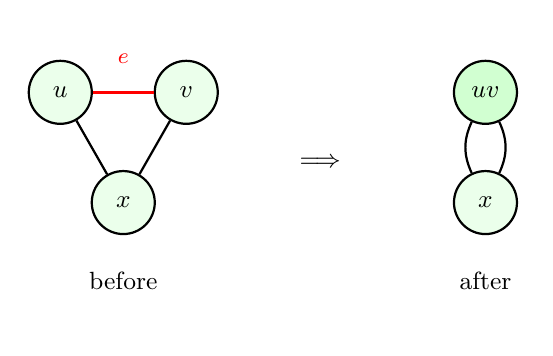
\begin{tikzpicture}[every node/.style={circle,draw,fill=green!8,minimum size=8mm,font=\small},thick]
  \node (a) at (0,1.4) {$u$};
  \node (b) at (1.6,1.4) {$v$};
  \node (c) at (0.8,0) {$x$};
  \draw[red,very thick] (a)--(b) node[midway,above,draw=none,fill=none,font=\footnotesize]{$e$};
  \draw (a)--(c); \draw (b)--(c);
  \node[draw=none,fill=none] at (0.8,-1) {before};
  \node[draw=none,fill=none] at (3.3,0.5) {$\Longrightarrow$};
  \node[fill=green!18] (uv) at (5.4,1.4) {$uv$};
  \node (c2) at (5.4,0) {$x$};
  \draw (uv) to[bend left=25] (c2);
  \draw (uv) to[bend right=25] (c2);
  \node[draw=none,fill=none] at (5.4,-1) {after};
\end{tikzpicture}
\caption{Contracting $e=\{u,v\}$. The two $x$-edges become a \emph{double} edge to the super-vertex $uv$; the copy of $e$ becomes a self-loop and is discarded. Multiplicities are preserved on purpose.}
\label{ch11:fig-contract}
\end{figure}

\begin{lemma}[Contraction preserves untouched cuts]\label{ch11:lem-contract}
Let $\Gph'=\Gph/e$ be $\Gph$ with edge $e=\{u,v\}$ contracted. There is a weight-preserving bijection between cuts of $\Gph'$ and cuts of $\Gph$ that do \emph{not} separate $u$ from $v$. In particular, the min-cut of $\Gph'$ is at least the min-cut of $\Gph$: $\lambda(\Gph')\ge\lambda(\Gph)$, with equality unless every min-cut of $\Gph$ separates $u$ and $v$.
\end{lemma}

\begin{proof}
A cut $(S',\bar S')$ of $\Gph'$ assigns the super-vertex $uv$ entirely to one side. Expand it to $\Gph$ by replacing $uv$ with both $u$ and $v$ on that same side; this is a cut of $\Gph$ that keeps $u,v$ together, and its crossing edges are in bijection with the crossing edges of $(S',\bar S')$ (the only edges that disappeared under contraction were copies of $e$, which never cross a cut keeping $u,v$ together). The map is reversible, hence a weight-preserving bijection. Cuts of $\Gph$ that separated $u$ from $v$ have no preimage, so $\Gph'$ has a subset of $\Gph$'s cuts; the minimum over a subset is no smaller.
\end{proof}

\subsection{The algorithm}

\begin{algorithm}[H]
\caption{\textsc{KargerContract}$(\Gph)$ --- one trial (unweighted multigraph)}
\label{ch11:alg-karger}
\DontPrintSemicolon
\KwIn{connected multigraph $\Gph=(V,E)$, $n=\abs V$}
\KwOut{a cut of $\Gph$ (its value is the number of surviving edges)}
\While{$\abs V > 2$}{
  pick an edge $e$ uniformly at random from the current edge multiset $E$\;
  $\Gph \gets \Gph / e$ \tcp*{contract: merge endpoints, keep multi-edges, drop loops}
}
\Return the cut given by the two remaining super-vertices (value $=\abs E$)\;
\end{algorithm}

For \emph{weighted} graphs, ``pick a uniformly random edge'' becomes ``pick edge $e$ with probability proportional to $w(e)$,'' and the surviving cut value is the total surviving weight. The analysis below is for the unweighted (multigraph) case; the weighted case follows by treating weight as parallel-edge multiplicity (or directly with the weighted sampling probabilities, see Exercise~\ref{ch11:ex-weighted}).

\begin{intuitionbox}
A min-cut has few edges by definition. A uniformly random edge is therefore \emph{unlikely} to be one of the precious min-cut edges --- most edges live inside the two sides, not across the cut. Each contraction of a non-cut edge merges two vertices that the min-cut keeps together, leaving the min-cut intact (Lemma~\ref{ch11:lem-contract}). If we are lucky enough to never contract a min-cut edge across all $n-2$ steps, the two survivors are exactly the two sides of the min-cut. The whole analysis is bounding the probability of that lucky streak.
\end{intuitionbox}

\subsection{Success probability}

Fix one particular minimum cut $C^\ast$ of weight $k=\lambda(\Gph)$ (there may be several; we only need one to survive). The trial \emph{succeeds for $C^\ast$} if it never contracts an edge of $C^\ast$.

\begin{lemma}[Min-degree bound]\label{ch11:lem-mindeg}
At every stage of contraction, a multigraph on $r$ super-vertices whose min-cut is still $\ge k$ has at least $rk/2$ edges; hence each vertex has degree $\ge k$ and a uniformly random edge crosses $C^\ast$ with probability $\le k/(rk/2)=2/r$.
\end{lemma}

\begin{proof}
Contraction never decreases the min-cut (Lemma~\ref{ch11:lem-contract}), so throughout the run every super-vertex has degree at least $k$ (isolating it is a cut, which costs $\ge k$). Summing degrees, $2\abs E=\sum_v \deg v \ge rk$, so $\abs E\ge rk/2$. The cut $C^\ast$ contributes exactly $k$ edges to the current multigraph as long as none has been contracted, so the chance the random edge is one of them is $k/\abs E \le k/(rk/2)=2/r$.
\end{proof}

\begin{theorem}[Karger success probability]\label{ch11:thm-karger}
A single run of Algorithm~\ref{ch11:alg-karger} returns the fixed min-cut $C^\ast$ with probability at least
\[
  \Pr[\text{success}] \;\ge\; \binom{n}{2}^{-1} \;=\; \frac{2}{n(n-1)}.
\]
\end{theorem}

\begin{proof}
Let $E_i$ be the event ``the $i$-th contraction does not destroy $C^\ast$,'' i.e.\ the chosen edge is not a $C^\ast$-edge. Before the $i$-th contraction there are $r=n-i+1$ vertices, so by Lemma~\ref{ch11:lem-mindeg},
\[
  \Pr[E_i \mid E_1\cap\cdots\cap E_{i-1}] \;\ge\; 1-\frac{2}{n-i+1}\;=\;\frac{n-i-1}{n-i+1}.
\]
The run succeeds iff all $n-2$ events occur. Multiply the conditional probabilities (telescoping product):
\[
  \Pr[\text{success}] \;\ge\; \prod_{i=1}^{n-2}\frac{n-i-1}{n-i+1}
  \;=\; \frac{n-2}{n}\cdot\frac{n-3}{n-1}\cdot\frac{n-4}{n-2}\cdots\frac{2}{4}\cdot\frac{1}{3}.
\]
Almost everything cancels: numerators $n-2,n-3,\dots,1$ against denominators $n,n-1,\dots,3$. What survives is $\dfrac{2\cdot 1}{n(n-1)}=\dbinom{n}{2}^{-1}$.
\end{proof}

\begin{connectionbox}
This proof is a pure exercise in conditional probability and the chain rule $\Pr[\bigcap E_i]=\prod \Pr[E_i\mid E_1\cap\cdots\cap E_{i-1}]$ --- exactly the machinery developed in the companion probability book. The telescoping product is the same algebraic move that appears in birthday-paradox and coupon-collector calculations. And Theorem~\ref{ch11:thm-karger} has a striking structural corollary below: an upper bound on the number of distinct min-cuts, obtained purely from the probability bound, not from any combinatorial enumeration.
\end{connectionbox}

\begin{corollary}[At most $\binom{n}{2}$ minimum cuts]\label{ch11:cor-count}
A graph on $n$ vertices has at most $\binom{n}{2}$ distinct minimum cuts.
\end{corollary}

\begin{proof}
For each distinct min-cut $C_j$, the events ``a single Karger run outputs $C_j$'' are disjoint (a run outputs exactly one cut). Each has probability $\ge\binom{n}{2}^{-1}$ by Theorem~\ref{ch11:thm-karger}. Disjoint events have probabilities summing to at most $1$, so the number of distinct min-cuts is at most $\binom{n}{2}$. This bound is tight: the cycle $C_n$ has exactly $\binom{n}{2}$ min-cuts (cut any two of its $n$ edges).
\end{proof}

\subsection{Amplification}

A success probability of $\sim 2/n^2$ sounds tiny, but independent repetition crushes the failure probability. Run the trial $T$ times and keep the lightest cut found. The probability that \emph{all} $T$ trials miss $C^\ast$ is at most $\big(1-\binom{n}{2}^{-1}\big)^T$. Using $1-x\le e^{-x}$,
\[
  \Pr[\text{all }T\text{ fail}] \;\le\; \Big(1-\tbinom{n}{2}^{-1}\Big)^{T}
  \;\le\; \exp\!\Big(-T\big/\tbinom{n}{2}\Big).
\]
Choosing $T = \binom{n}{2}\ln n \approx \tfrac12 n^2\ln n$ drives the failure probability below $e^{-\ln n}=1/n$; choosing $T=c\,\binom{n}{2}\ln n$ gives failure $\le n^{-c}$ --- high probability for any constant $c$.

\begin{complexitybox}
One trial does $n-2$ contractions; a careful adjacency-matrix implementation makes each contraction $\Oh(n)$, so a trial is $\Oh(n^2)$. Amplifying to failure $\le 1/n$ needs $\Oh(n^2\log n)$ trials, for a total of
\[
  \Oh(n^2)\cdot\Oh(n^2\log n) \;=\; \Oh(n^4\log n).
\]
That is worse than Stoer--Wagner. The fix --- Karger--Stein --- is to notice that the early contractions are very safe and only the late ones are dangerous, so we should not redo the safe prefix every trial.
\end{complexitybox}

\section{Karger--Stein: recurse where it is risky}

Look again at the per-step survival probability $1-2/r$. When $r$ is large (early on), each contraction is nearly safe; when $r$ shrinks toward $2$, the factors $1-2/r$ become small and that is where most failures happen. So contracting all the way down and starting over wastes the safe early work. Karger and Stein's idea: contract down to a moderate size where success is still about $1/2$, then \emph{branch} --- run two independent continuations and recurse --- so that the dangerous tail gets two chances each time.

\subsection{The partial-contraction guarantee}

\begin{lemma}[Surviving to $t$ vertices]\label{ch11:lem-survive}
Starting from $n$ vertices and contracting random edges until $t$ vertices remain, the fixed min-cut $C^\ast$ survives with probability at least
\[
  \Pr[\text{survive to }t] \;\ge\; \frac{\binom{t}{2}}{\binom{n}{2}} \;=\; \frac{t(t-1)}{n(n-1)}.
\]
\end{lemma}

\begin{proof}
Same telescoping product as Theorem~\ref{ch11:thm-karger}, but stop after $n-t$ contractions (when $t$ vertices remain):
\[
  \prod_{i=1}^{n-t}\Big(1-\frac{2}{n-i+1}\Big)
  = \prod_{r=t+1}^{n}\frac{r-2}{r}
  = \frac{(t-1)t}{n(n-1)} = \frac{\binom{t}{2}}{\binom{n}{2}}.
\]
\end{proof}

Choosing $t=\lceil 1+n/\sqrt2\rceil$ makes $\binom{t}{2}/\binom{n}{2}\ge \tfrac12$: contracting down to a $1/\sqrt2$ fraction of the vertices keeps the min-cut alive with probability at least one half.

\subsection{The recursion}

\begin{algorithm}[H]
\caption{\textsc{KargerStein}$(\Gph)$}
\label{ch11:alg-ks}
\DontPrintSemicolon
\KwIn{multigraph $\Gph$ with $n=\abs V$ vertices}
\KwOut{a cut of $\Gph$; with the recursion it is the min-cut w.h.p.}
\If{$n \le 6$}{
  \Return min-cut found by brute force (e.g.\ Stoer--Wagner) on $\Gph$\;
}
$t \gets \big\lceil 1 + n/\sqrt2\,\big\rceil$\;
$\Gph_1 \gets$ contract random edges of $\Gph$ down to $t$ vertices\;
$\Gph_2 \gets$ contract random edges of $\Gph$ down to $t$ vertices \tcp*{independent of $\Gph_1$}
\Return $\min\big(\textsc{KargerStein}(\Gph_1),\ \textsc{KargerStein}(\Gph_2)\big)$\;
\end{algorithm}

\begin{intuitionbox}
The recursion tree is a binary tree of depth $\Oh(\log n)$. Each node shrinks its graph by a factor $\sqrt2$ and survives with probability $\ge 1/2$, then hands two independent copies to its children. Two children, each succeeding with probability $\ge 1/2$ on a problem half the ``risk'' --- that is exactly the structure that makes the overall success probability decay only polynomially with depth instead of exponentially with the number of contractions.
\end{intuitionbox}

\subsection{Running time}

Let $T(n)$ be the time for one call. Contracting from $n$ to $t\approx n/\sqrt2$ vertices costs $\Oh(n^2)$ (each of $\Oh(n)$ contractions is $\Oh(n)$), done twice, and there are two recursive calls on graphs of size $\approx n/\sqrt2$:
\[
  T(n) = 2\,T\!\Big(\tfrac{n}{\sqrt2}+1\Big) + \Oh(n^2).
\]
By the master theorem with $a=2$, $b=\sqrt2$, so $\log_b a = \log_{\sqrt2}2 = 2$, and the work per level $\Oh(n^2)$ matches $n^{\log_b a}=n^2$: the balanced case. Hence
\[
  T(n) = \Oh(n^2\log n).
\]
The recursion tree has $\Oh(n^2)$ leaves and $\Oh(\log n)$ levels, $\Oh(n^2)$ total work per level.

\subsection{Success probability of the recursion}

\begin{theorem}[Karger--Stein success]\label{ch11:thm-ks}
Algorithm~\ref{ch11:alg-ks} finds the min-cut with probability $\Om\!\big(1/\log n\big)$.
\end{theorem}

\begin{proof}
Let $P(n)$ lower-bound the probability that a call on $n$ vertices finds $C^\ast$. Each of the two children succeeds if (a) the partial contraction to $t$ vertices preserves $C^\ast$ --- probability $\ge 1/2$ by the choice of $t$ --- and (b) the recursive call then finds it --- probability $\ge P(t)$. So a single child succeeds with probability $\ge \tfrac12 P(t)$, and the parent succeeds if \emph{either} child does:
\[
  P(n) \;\ge\; 1 - \Big(1 - \tfrac12 P(t)\Big)^2, \qquad t\approx \tfrac{n}{\sqrt2}.
\]
Index the recursion by depth: let $p_d$ be the success probability at a node $d$ levels above the leaves, with $p_0=\Th(1)$ (the brute-force base case is exact). Expanding the recurrence, $p_d \ge p_{d-1} - \tfrac14 p_{d-1}^2$. Put $q_d=1/p_d$; from $p=p'-\tfrac14 p'^2$ one has $1/p = 1/p' + 1/(4-p') \le 1/p' + 1/3$ for $p'\in(0,1]$, so $q_d \le q_{d-1}+\tfrac13$. Therefore $q_d \le q_0 + d/3 = \Oh(\log n)$ since $d=\Oh(\log n)$, giving $p_d = \Om(1/\log n)$.
\end{proof}

So a \emph{single} Karger--Stein run succeeds with probability $\Om(1/\log n)$. Repeating it $\Oh(\log^2 n)$ times and keeping the best cut pushes the failure probability below $1/n$ (each run fails with probability $\le 1-c/\log n\le e^{-c/\log n}$; raising to the $\Oh(\log^2 n)$ power gives $e^{-c\log n}=n^{-c}$), for a total of
\[
  \Oh(n^2\log n)\cdot \Oh(\log^2 n) \;=\; \Oh(n^2\log^3 n).
\]

\begin{complexitybox}
\begin{tabular}{lll}
\toprule
Algorithm & Time & Guarantee \\
\midrule
Karger, one trial & $\Oh(n^2)$ & finds min-cut w.p.\ $\ge \binom{n}{2}^{-1}$ \\
Karger, amplified & $\Oh(n^4\log n)$ & w.h.p.\ ($\ge 1-1/n$) \\
Karger--Stein, one run & $\Oh(n^2\log n)$ & w.p.\ $\Om(1/\log n)$ \\
Karger--Stein, amplified & $\Oh(n^2\log^3 n)$ & w.h.p.\ \\
Stoer--Wagner & $\Oh(nm+n^2\log n)$ & deterministic, exact \\
Karger tree-packing (2000) & $\Oh(m\log^3 n)$ & w.h.p.\ \\
\bottomrule
\end{tabular}\\[0.4em]
Karger--Stein at $\Oh(n^2\log^3 n)$ on dense graphs beats both naive flow ($\Oh(mn^2)$) and Stoer--Wagner's $\Oh(n^3)$.
\end{complexitybox}

\begin{trapbox}
The single most common Karger bug is \emph{merging parallel edges} during contraction. If you collapse the two $x$-edges of Figure~\ref{ch11:fig-contract} into one, you destroy the multiplicities that make a random edge land across the min-cut with probability $k/\abs E$ --- the entire probability analysis assumes uniform sampling over the multiset. Use an adjacency \emph{matrix of counts} (or weights) and add them; never deduplicate. A second trap: in Karger--Stein, the two recursive branches must contract \emph{independently} from the same parent graph --- if you reuse one contracted graph for both branches you lose the second chance and the success probability collapses back to Karger's $1/n^2$.
\end{trapbox}

\subsection{Tracing Karger by hand}

Take a tiny example where we can compute everything: the $4$-cycle $C_4$ with vertices $1,2,3,4$ and edges $12,23,34,41$, all weight $1$. Its min-cut is $2$ (removing $12$ and $34$ separates $\{1,4\}$ from $\{2,3\}$, for instance). By Corollary~\ref{ch11:cor-count} there are at most $\binom42=6$ min-cuts; for $C_4$ every pair of edges removed disconnects it, so there are exactly $6$, hitting the bound.

One trial: $n=4$, we contract twice.
\begin{itemize}
  \item \textbf{Step 1} ($r=4$, $4$ edges). Pick a uniform edge, say $23$. Contract: super-vertex $23$, edges become $1{-}23$ (the old $12$), $23{-}4$ (the old $34$), $4{-}1$. Now $3$ vertices $\{1, 23, 4\}$ forming a triangle, $3$ edges.
  \item \textbf{Step 2} ($r=3$, $3$ edges). Pick a uniform edge, say $4{-}1$. Contract: super-vertex $14$. Two vertices $\{14, 23\}$ with edges $14{-}23$: the old $1{-}23$ and $23{-}4$, so a \emph{double} edge. Surviving cut value $=2$. Success --- this equals $\lambda=2$, separating $\{1,4\}$ from $\{2,3\}$.
\end{itemize}
On $C_4$ every trial returns value $2$, because every $2$-edge removal is a min-cut. Theorem~\ref{ch11:thm-karger} promises success $\ge 1/\binom42 = 1/6$ for each \emph{fixed} cut; summed over the $6$ min-cuts that (correctly) permits total success probability up to $1$.

\begin{labbox}
Build a graph where Karger genuinely fails sometimes: take two triangles $\{a,b,c\}$ and $\{x,y,z\}$ joined by a single edge $c{-}x$. The unique min-cut is $\{c,x\}$ (value $1$). Trace: a trial succeeds only if the last surviving edge is $c{-}x$, i.e.\ it never contracts $c{-}x$ and collapses each triangle first. Estimate the success probability by hand and compare to the $\binom72^{-1}=1/21$ guarantee --- you should beat the bound comfortably, since the bound is worst-case.
\end{labbox}

\section{Applications}

\begin{applicationbox}
\textbf{Network reliability.} The edge connectivity $\lambda(\Gph)$ is the number of link failures a network can tolerate before splitting. Telecom and data-center fabrics are designed so $\lambda$ exceeds a target; global min-cut finds the weakest seam to reinforce. Karger's contraction view also yields the fastest known algorithms for estimating all-terminal network \emph{reliability} (the probability a random subgraph stays connected), because near-minimum cuts dominate the failure probability and Corollary~\ref{ch11:cor-count} extends to bound the number of \emph{near}-minimum cuts.

\textbf{Image segmentation and clustering.} Treat pixels (or data points) as vertices and put a heavy edge between similar neighbors. A light global cut separates dissimilar regions; this is the combinatorial cousin of the spectral ``normalized cut'' and the starting point for graph-based segmentation. When you want balanced sides you switch to sparsest/normalized cut (the Cheeger and spectral chapters), but unbalanced global min-cut is the exact, polynomial baseline.

\textbf{VLSI and partitioning.} Splitting a circuit netlist across two chips while cutting the fewest wires is a min-cut. The unconstrained version is global min-cut; adding balance constraints makes it NP-hard, which is why heuristics (and spectral relaxations) take over.

\textbf{A structural bound.} Corollary~\ref{ch11:cor-count} --- at most $\binom n2$ min-cuts --- is itself the application: it underlies cut-sparsification, the analysis of randomized algorithms, and the fact that you can store \emph{all} min-cuts compactly in the cactus representation.
\end{applicationbox}

\begin{connectionbox}
Global min-cut sits at a crossroads of this book.
\begin{itemize}
  \item \textbf{Max-flow (Chapter~12).} The naive $n-1$ flow reduction and Hao--Orlin connect global cut to $s$--$t$ duality; Stoer--Wagner is what you reach for to \emph{avoid} flow entirely.
  \item \textbf{Spectral graph theory and the Laplacian $\Lap$.} The min-cut is the combinatorial extreme; the second Laplacian eigenvalue $\lambda_2(\Lap)$ (Fiedler value) controls the \emph{balanced} cut via Cheeger's inequality. Random contraction and random walks share the same ``most edges are internal'' intuition that makes $\Lap$'s spectrum reveal cuts.
  \item \textbf{Probability book.} Theorem~\ref{ch11:thm-karger} and Lemma~\ref{ch11:lem-survive} are textbook conditional-probability chain-rule arguments; the amplification step is the union/independence bound $1-(1-p)^T\ge 1-e^{-pT}$ used throughout randomized algorithms.
\end{itemize}
\end{connectionbox}

\section*{Summary}

Global min-cut asks for the cheapest split of a graph with no fixed terminals. You can pay $n-1$ max-flows, but two direct algorithms are better and far more instructive. Stoer--Wagner grows maximum-adjacency orderings; the trailing two vertices of each ordering give a true $s$--$t$ min-cut (Lemma~\ref{ch11:lem-phase}), and contracting them across $n-1$ phases sweeps out the global optimum deterministically in $\Oh(nm+n^2\log n)$. Karger contracts a uniformly random edge until two vertices remain; a fixed min-cut survives with probability $\ge\binom n2^{-1}$ (Theorem~\ref{ch11:thm-karger}), which both gives a randomized algorithm and proves there are at most $\binom n2$ min-cuts. Karger--Stein spends two independent recursive continuations on the risky tail of the contraction, reaching $\Oh(n^2\log^3 n)$ with high probability --- one of the prettiest divide-and-conquer-with-randomness arguments in the field.

\section{Exercises}

\begin{exercise}[Implement Stoer--Wagner]\label{ch11:ex-implsw}
Implement the dense $\Oh(n^3)$ version with an $n\times n$ weight matrix and a boolean ``merged'' array. Run it on Figure~\ref{ch11:fig-running} and confirm it returns $4$ with side $\{3,4,7,8\}$. Then add cut recovery: maintain for each super-vertex the list of original vertices it absorbed, and output the actual partition.
\end{exercise}

\begin{exercise}[Implement Karger and Karger--Stein]\label{ch11:ex-implkarger}
Implement Karger with a count-matrix contraction in $\Oh(n^2)$ per trial. Empirically measure the success rate over many trials on $C_n$ for $n=5,\dots,20$ and compare to $\binom n2^{-1}$. Then implement Karger--Stein and verify the success rate is $\Om(1/\log n)$ per run.
\end{exercise}

\begin{exercise}[The greedy lemma is local]\label{ch11:ex-tight}
In Lemma~\ref{ch11:lem-phase} we only proved the cut-of-the-phase is an $s$--$t$ min-cut for the \emph{last two} vertices. Give a small weighted graph and an MA-order in which the first cut-of-the-phase is \emph{not} a global min-cut, so the algorithm genuinely needs more than one phase to find $\lambda$.
\end{exercise}

\begin{exercise}[Counting min-cuts is tight]\label{ch11:ex-cycle}
Prove the cycle $C_n$ has exactly $\binom n2$ distinct minimum cuts, each of value $2$, matching Corollary~\ref{ch11:cor-count}. Then exhibit a graph with strictly fewer than $\binom n2$ min-cuts, confirming the bound is an inequality in general.
\end{exercise}

\begin{exercise}[Weighted Karger]\label{ch11:ex-weighted}
Extend Algorithm~\ref{ch11:alg-karger} to weighted graphs by sampling edge $e$ with probability $w(e)/\sum_f w(f)$. Prove that Theorem~\ref{ch11:thm-karger} still holds with $k=\lambda(\Gph)$ the weighted min-cut. (Hint: redo Lemma~\ref{ch11:lem-mindeg} with weighted degrees; the bound $2/r$ on the probability of cutting $C^\ast$ is unchanged.)
\end{exercise}

\begin{exercise}[Min-cut from max-flow, carefully]\label{ch11:ex-flow}
Show that $\lambda(\Gph)=\min_{t\neq s}(\text{$s$--$t$ min-cut})$ for any fixed $s$. Why is it correct to fix $s$ and vary only $t$, rather than ranging over all $\binom n2$ pairs? Then argue that on an undirected graph you need at most $n-1$ flow computations, and sketch why Gomory--Hu trees encode all $\binom n2$ pairwise min-cuts in only $n-1$ flows.
\end{exercise}

\begin{exercise}[Break a buggy contraction]\label{ch11:ex-break}
Suppose a colleague's Karger implementation merges parallel edges (keeps each neighbor relation as a single weight-$1$ edge, discarding multiplicity). Construct a graph on which this bug makes the algorithm return the min-cut with probability bounded \emph{away} from the correct $\binom n2^{-1}$, or where it systematically returns the wrong value. Explain precisely which step of Lemma~\ref{ch11:lem-mindeg} fails.
\end{exercise}

\begin{exercise}[Near-minimum cuts]\label{ch11:ex-near}
Generalize Lemma~\ref{ch11:lem-survive}: show that for any $\alpha\ge 1$, the number of cuts of value at most $\alpha\lambda(\Gph)$ is $\Oh(n^{2\alpha})$. (Hint: stop the contraction earlier, bound the survival probability of a fixed $\alpha$-near-minimum cut, then use the disjointness argument of Corollary~\ref{ch11:cor-count}.)
\end{exercise}

\begin{exercise}[Which cut does Stoer--Wagner find?]\label{ch11:ex-which}
Stoer--Wagner returns \emph{a} min-cut; which one if there are several? Run it on $C_6$ (six min-cuts) under different start vertices and tie-breaking rules, and characterize which of the six it reports. Does the choice of start vertex change the returned \emph{value}? Should it?
\end{exercise}

\begin{exercise}[A lower-bound intuition]\label{ch11:ex-lower}
Argue informally why any correct deterministic global min-cut algorithm that only queries edge weights must, in the worst case, ``look at'' $\Om(m)$ edges, and why Stoer--Wagner's $\Oh(nm+n^2\log n)$ is therefore within a near-linear-in-$n$ factor of an obvious barrier. (This is intuition, not a formal lower bound --- formal lower bounds for min-cut are subtle.)
\end{exercise}
